\section{Gaussian Mixture Models}

K-means clustering is a form of hard clustering, where each data point is assigned to exactly one cluster. However, in some cases, soft clustering—where data points can belong to multiple clusters with varying degrees of membership—provides a better model in practice. A Gaussian Mixture Model (GMM) assumes a linear superposition of Gaussian components, offering a richer class of density models than a single Gaussian distribution.

In essence, rather than assuming that all data points are generated by a single Gaussian distribution, we assume that the data is generated by a mixture of \( K \) different Gaussian distributions, where each Gaussian represents a different component in the mixture.

For a single sample, the Gaussian Mixture Model can be expressed as a weighted sum of these individual Gaussian distributions:
\begin{align*}
	p(\mathbf{x}) &= \sum_\rvz p(\rvz)p(\rvx|\rvz) \\ 
				  &= \sum_{k=1}^{K} \pi_k \mathcal{N}(\mathbf{x} | \boldsymbol{\mu}_k, \boldsymbol{\Sigma}_k)
\end{align*}
Here, \( \mathbf{x} \) is a data point, \( \pi_k \) represents the mixing coefficients, \( \mathcal{N}(\mathbf{x} | \boldsymbol{\mu}_k, \boldsymbol{\Sigma}_k) \) is a Gaussian distribution with mean \( \boldsymbol{\mu}_k \) and covariance \( \boldsymbol{\Sigma}_k \), and \( K \) is the number of Gaussian components.

A key quantity in GMMs is the conditional probability of \( \mathbf{z} \) given \( \mathbf{x} \), denoted as \( p(z_k = 1 | \mathbf{x}) \) or \( \gamma(z_k) \). This is also known as the responsibility or assignment probability, which represents the probability that a given data point \( \mathbf{x} \) belongs to component \( k \) of the mixture. Essentially, this can be thought of as the \textbf{classification result} for \( \mathbf{x} \).

This responsibility is updated using Bayes' Theorem, and can be expressed as:
\begin{align*}
\gamma(z_k) \equiv p(z_k=1|\mathbf{x}) & \equiv \frac{p(z_k=1)p(\mathbf{x}|z_k=1)}{\sum_{j=1}^{K}p(z_j=1)p(\mathbf{x}|z_j=1)} \\
& = \frac{\pi_k\mathcal{N}(\mathbf{x}|\boldsymbol{\mu}_k, \boldsymbol{\Sigma}_k)}{\sum_{j=1}^{K} \pi_j\mathcal{N}(\mathbf{x}|\boldsymbol{\mu}_j, \boldsymbol{\Sigma}_j)}
\end{align*}

In this expression, \( \pi_k \) is the prior probability (or mixing coefficient) for component \( k \), and \( \mathcal{N}(\mathbf{x} | \boldsymbol{\mu}_k, \boldsymbol{\Sigma}_k) \) is the likelihood of the data point \( \mathbf{x} \) under the Gaussian distribution corresponding to component \( k \). The denominator is a normalization factor that ensures the responsibilities sum to 1 across all components for a given data point.

This framework allows for a soft classification of data points, where each point is associated with a probability of belonging to each cluster, rather than being strictly assigned to a single cluster as in K-means.

\subsection{Maximum Likelihood}
Suppose we have a data set of observations $\mathbf{X}=\{\mathbf{x}_1,\dots,\mathbf{x}_n\}^{T}\in\mathbb{R}^{N\times D}$ and we want to model the data distribution $p(\mathbf{X})$ using GMM. Assuming the data is independent and identically distributed (i.i.d.), the likelihood of the entire dataset can be expressed as:
\begin{align*}
	p(\mathbf{X}|\boldsymbol{\pi},\boldsymbol{\mu},\boldsymbol{\Sigma}) =\prod_{n=1}^{N}\left(\sum_{k=1}^{K}\pi_k\mathcal{N}(\mathbf{x}_n|\boldsymbol{\mu}_k, \boldsymbol{\Sigma}_k)\right).
\end{align*}
To simplify the optimization process, we consider the log-likelihood function, which is given by:
\begin{align*}
	\ln p(\mathbf{X}|\boldsymbol{\pi},\boldsymbol{\mu},\boldsymbol{\Sigma}) &= \sum_{n=1}^{N}\ln \Bigg(\sum_{k=1}^{K}\pi_k\mathcal{N}(\mathbf{x}_n|\boldsymbol{\mu}_k, \boldsymbol{\Sigma}_k)\Bigg)
\end{align*}
To solve the Maximum Likelihood Estimation (MLE) for Gaussian Mixture Models (GMMs), we typically consider the iterative \textit{Expectation-Maximization} (EM) algorithm due to the non-convex nature of the problem. Before discussing how to maximize the likelihood, it is important to emphasize two significant issues that arise in GMMs: \textit{singularities} and \textit{identifiability}.

\paragraph{Singularity} A major challenge in applying the maximum likelihood framework to Gaussian Mixture Models is the presence of singularities. This problem arises because the likelihood function can become unbounded under certain conditions, leading to an ill-posed optimization problem.

For simplicity, consider a Gaussian mixture model where each component has a covariance matrix of the form \( \Sigma_k = \sigma^2_k I \), where \( I \) is the identity matrix. Suppose one of the mixture components, say the \( j \)-th component, has its mean \( \boldsymbol{\mu}_j \) exactly equal to one of the data points \( \mathbf{x}_n \), so that \( \boldsymbol{\mu}_j = \mathbf{x}_n \) for some value of \( n \). The contribution of this data point to the likelihood function would then be:
\begin{align*}
	\mathcal{N}(\mathbf{x}_n | \mathbf{x}_n, \sigma^2_j I) = \frac{1}{\sqrt{2\pi} \sigma_j} \cdot \exp^0
\end{align*}
As \( \sigma_j \) approaches 0, this term goes to infinity, causing the log-likelihood function to also diverge to infinity. Therefore, maximizing the log-likelihood function becomes an ill-posed problem because such singularities can always be present. These singularities occur whenever one of the Gaussian components \textbf{collapses} onto a specific data point, leading to a covariance matrix with a determinant approaching zero. This issue did not arise with a single Gaussian distribution because the variance cannot be zero by definition.

\paragraph{Identifiability} Another issue in finding MLE solutions for GMMs is related to identifiability. For any given maximum likelihood solution, a GMM with \( K \) components has a total of \( K! \) equivalent solutions. This arises from the fact that the \( K! \) different ways of permuting the \( K \) sets of parameters (means, covariances, and mixing coefficients) yield the same likelihood.

In other words, for any point in the parameter space that represents a maximum likelihood solution, there are \( K! - 1 \) additional points that produce exactly the same probability distribution. This lack of identifiability means that the solution is not unique, complicating both the interpretation of the model and the optimization process.

\subsection{Expectation Maximization for GMM}

The goal of the Expectation-Maximization (EM) algorithm is to find maximum likelihood solutions for models that involve latent variables.
\begin{itemize}
	\item Suppose that directly optimizing the likelihood $p(\mathbf{X}|\boldsymbol{\theta})$ is difficult.
	\item However, it is easier to optimize the complete-data likelihood function $p(\mathbf{X}, \mathbf{Z}|\boldsymbol{\theta})$ as as discussed in the previous sections.
	\item In such cases, we can use the \textbf{EM algorithm}. EM algorithm is a general technique for finding maximum likelihood solutions in latent variable models. 
\end{itemize}
Let's begin by writing down the conditions that must be satisfied at a maximum of the likelihood function. By setting the derivatives of $\ln p(\mathbf{X}|\boldsymbol{\pi},\boldsymbol{\mu},\boldsymbol{\Sigma})$ with respect to the means $\boldsymbol{\mu}_k$ of the Gaussian components to zero, we obtain
\begin{align*}
	0 = -\sum_{n=1}^N\frac{\pi_k\mathcal{N}(\mathbf{x}|\boldsymbol{\mu}_k, \boldsymbol{\Sigma}_k)}{\sum_{j=1}^{K} \pi_j\mathcal{N}(\mathbf{x}|\boldsymbol{\mu}_j, \boldsymbol{\Sigma}_j)}\boldsymbol{\Sigma}_k(\mathbf{x}_n-\boldsymbol{\mu}_k)
\end{align*}
Multiplying by $\boldsymbol{\Sigma}_k^{-1}$ (which we assume to be non-singular) and rearranging we obtain
\begin{align*}
	\boldsymbol{\mu}_k = \frac{1}{N_k}\sum_{n=1}^{N}\gamma(z_{nk})\mathbf{x}_n, 
\end{align*}
where we have defined
\begin{align*}
	N_k = \sum_{n=1}^{N}\gamma(z_{nk}).
\end{align*}
We can interpret $N_k$ as the effective number of points assigned to cluster $k$. We can obtain the MLE solutions for other variables similarly.
\begin{algorithm}
	Initialize the means $\boldsymbol{\mu}_k$, covariances $\boldsymbol{\Sigma}_k$ and mixing coefficients $\pi_k$ and evaluate the initial value of the log likelihood.\\
	\For{n}{
		E-step: evaluate the responsibilities of $\mathbf{x}_n$ based on the current parameter values with the given parameters
		$$ \gamma(z_{nk})= p(z_k=1|\mathbf{x}_n) =  \frac{\pi_k\mathcal{N}(\mathbf{x}_n|\boldsymbol{\mu}_k, \boldsymbol{\Sigma}_k)}{\sum_{j=1}^{K} \pi_j\mathcal{N}(\mathbf{x}_n|\boldsymbol{\mu}_j, \boldsymbol{\Sigma}_j)}$$\\
		where $z_{nk}$ denote the $k$-th component of $\mathbf{z}_n$\\
		M-step: maximize expectation
		\begin{itemize}
			\item $\boldsymbol{\mu}_k^{\textrm{new}} = \frac{1}{N_k}\sum_{n=1}^{N}\gamma(z_{nk})\mathbf{x}_n$
			\item $\boldsymbol{\Sigma}_k^{\textrm{new}} = \frac{1}{N_k}\sum_{n=1}^{N}\gamma(z_{nk})(\mathbf{x}_n-\boldsymbol{\mu}_k^{\textrm{new}})(\mathbf{x}_n-\boldsymbol{\mu}_k^{\textrm{new}})^T$
			\item $\pi_k^{\textrm{new}} = p(z_k=1) = \frac{N_k}{N}$
		\end{itemize}
	Evaluate the log likelihood to check for convergence of parameters
	$$\textrm{ln}p(\mathbf{X}|\boldsymbol{\pi},\boldsymbol{\mu},\boldsymbol{\Sigma}) = \sum_{n=1}^{N}\textrm{ln}\Bigg(\sum_{k=1}^{K}\pi_k\mathcal{N}(\mathbf{x}_n|\boldsymbol{\mu}_k, \boldsymbol{\Sigma}_k)\Bigg)$$
	}
	\caption{EM algorithm for GMM}
\end{algorithm}
	\begin{figure}[h]
	\begin{center}
		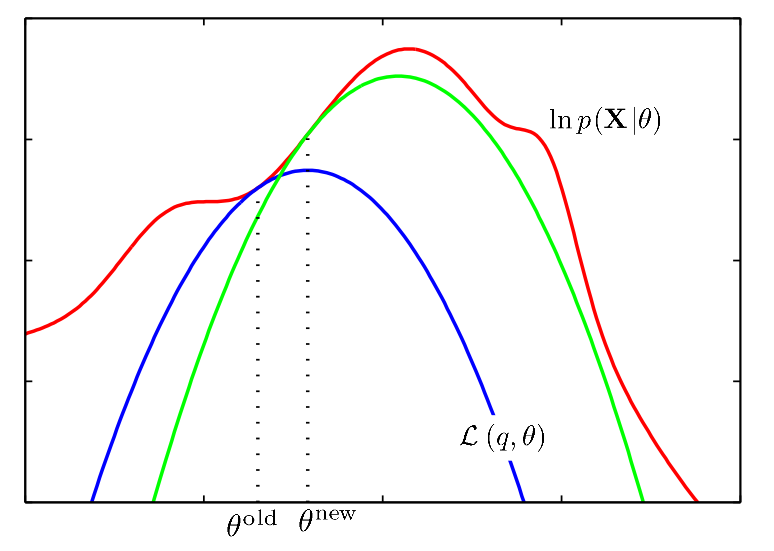
\includegraphics[scale=0.25]{./images/generative/em_update.png}
	\end{center}
	\caption{M-step of EM algorithm}
	\label{fig:em2}
\end{figure}

\section{Alternative View of EM}
The goal of the EM algorithm is to find maximum likelihood (loglikelihood) solutions for models having latent variables.
$$\ln p(X|\theta) = ln\sum_Z p(X,Z|\theta).$$
We are not given the complete data set ${X, Z}$, but only the incomplete data $X$. Our state of knowledge of the values of the latent variables
in $Z$ is given only by the posterior distribution $p(Z|X, \theta)$. Because we cannot use the complete-data log likelihood function, we consider instead its expected value under the posterior distribution of the latent variable, which corresponds (as we shall see) to the E-step of the EM algorithm.

In the subsequent M-step, we maximize this expectation. If the current estimate for the parameters is denoted $\theta_{old}$, then a pair of successive E- and M-steps gives rise to a revised estimate $\theta^{new}$.

The algorithm is initialized by choosing some starting value for the parameters $\theta_0$. The use of the expectation may seem somewhat arbitrary.

In the E-step, we use the current parameter values $\theta^{old}$ to find the posterior distribution of the latent variables given by $p(Z|X, \theta^{old})$. We then use this posterior distribution to find the \textbf{expectation of the complete-data log likelihood function} evaluated for some general parameter value $\theta$. In other words, this is a expectation over a some function. This expectation, denoted $Q(\theta, \theta^{old})$, is given by 
\begin{align*}
	Q(\theta, \theta^{old}) = \sum_Z p(Z|X, \theta^{old})\ln p(X,Z|\theta).
\end{align*}
In the M-step, we determine the revised parameter estimate $\theta^{new}$ by maximizing this function
$$\theta^{new}=\argmax Q(\theta, \theta^{old}).$$


\begin{algorithm}
The goal is to maximize the likelihood function $p(X|\theta)$ with respect to $\theta$ given a joint distribution $p(X, Z|\theta)$.\\
1. Init $\theta^{old}$\\
2. E-Step: evaluate $p(Z|X, \theta^{old})$ \\
3. M-Step: evaluate $\theta^{new}$ given by 
$$\theta^{new} = \argmax Q(\theta, \theta^{old}),$$
where
$$Q(\theta, \theta^{old}) = \sum_Z p(Z|X, \theta^{old})\ln p(X,Z|\theta).$$
4. Check for convergence of either the log likelihood or the parameter values. If the convergence criterion is not satisfied, then let
$$\theta^{old}\leftarrow \theta^{new}.$$
Return to the step 2. 
\caption{General EM algorithm}
\end{algorithm}

